%\documentclass[10pt]{article}
\documentclass[twocolumn,showpacs,preprintnumbers,amsmath,amssymb]{revtex4}
%\documentclass[preprint,showpacs,preprintnumbers,amsmath,amssymb]{revtex4}

% Some other (several out of many) possibilities
%\documentclass[preprint,aps]{revtex4}
%\documentclass[preprint,aps,draft]{revtex4}
%\documentclass[prb]{revtex4}% Physical Review B
\usepackage{CJK}
\usepackage{graphicx}% Include figure files
\usepackage{dcolumn}% Align table columns on decimal point
\usepackage{bm}% bold math

%\def\REF#1{\par\hangindent\parindent\indent\llap{#1\enspace}\ignorespaces}
%%%%%%%%%%%%%%%      define  enviroment     %%%%%%%%%%%%%%%%%%%%%
%\newcommand{\cc}[1]{$^{#1}$}
%\usepackage{psfig,epsfig}
%\def\kaishu{\CJKfamily{kai}} \def\heiti{\CJKfamily{hei}}
%\def\songti{\CJKfamily{song}} %%% \def\fangsong{\CJKfamily{fang}}
% \def\fangsong{\CJKfamily{song}}
 %\def\chbd{\begin{document} \begin{CJK*}{GB}{}}
%\def\ched{\end{CJK*} \end{document}}

%\nofiles
\def\btbl{\begin{tabular}} \def\etbl{\end{tabular}}
\def\bcc{\begin{center}} \def\ecc{\end{center}}
\def\beq{\begin{equation}} \def\eeq{\end{equation}}
\def\btbl{\begin{tabular}} \def\etbl{\end{tabular}}
\def\CME{{\footnotesize CME}} \def\CSE{{\footnotesize CSE}}
\def\RQMD{{\footnotesize RQMD}} \def\QCD{{\footnotesize QCD}}
\def\CERN{{\footnotesize CERN}} \def\SPS{{\footnotesize SPS}}
\def\LHC{{\footnotesize LHC}} \def\QGP{{\footnotesize QGP}}
\def\NA49{{\footnotesize NA49}} \def\NA35{{\footnotesize NA35}}
\def\RHIC{{\footnotesize RHIC}} \def\PHOBOS{{\footnotesize PHOBOS}}
\def\FRITIOF{{\footnotesize FRITIOF}}
\def\GeV{{\footnotesize GeV}} \def\DIS{{\footnotesize DIS}}
\def\BNL{{\footnotesize BNL}} \def\AGS{{\footnotesize AGS}}
\def\RHIC{{\footnotesize RHIC}} \def\LHC{{\footnotesize LHC}}
\def\MAC{{\footnotesize MAC}} \def\LET{{\footnotesize LET}}
\def\MITCH{{\footnotesize MITCH}} \def\CAMAC{{\footnotesize CAMAC}}
\def\DA{{\footnotesize DA}} \def\VME{{\footnotesize VME}}
\def\ADC{{\footnotesize ADC}} \def\TDC{{\footnotesize TDC}}
\def\MIC{{\footnotesize MIC}} \def\FSCC{{\footnotesize FSCC}}
\def\PMT{{\footnotesize PMT}} \def\TOF{{\footnotesize TOF}}
\def\TOP{{\footnotesize TOP}} \def\BOT{{\footnotesize BOT}}
\def\SMIT{{\footnotesize SMIT}} \def\SLEW{{\footnotesize SLEW}}
\def\START{{\footnotesize START}}
\def\Y{{\footnotesize Y}}\def\HCT{{\footnotesize HCT}}
\def\AGS{{\footnotesize AGS}} \def\KMW{{\footnotesize KMW}}
\def\GEANT{{\footnotesize GEANT}}\def\AMPT{{\footnotesize AMPT}}
\def\d{\rm d}
%\usepackage{graphicx}
%\usepackage{amssymb}
%\usepackage{epsfig}
%%%%%%%%%%%%%%%%%%%%%%%%%%%%%%%%%%%%%%%%%%%%%%%%%%
%                                                %
%    BEGINNING OF TEXT                           %
%                                                %
%%%%%%%%%%%%%%%%%%%%%%%%%%%%%%%%%%%%%%%%%%%%%%%%%%

\begin{document}
\title{Study on Chiral Charge Separation Effect in Relativistic Heavy-ion Collisions}


\author{Sheng-Qin Feng$^{1,2,3}$}
\email{fengsq@ctgu.edu.cn}
\author{Lei Pei$^{1}$}
\author{Fei ~Sun$^{1}$}
\author{Yang Zhong$^{1}$}
\author{Xin Ai$^{1}$}
\author{Zhong-Bao Yin$^{2}$}


\affiliation{$^1$ College of Science, China Three Gorges University, Yichang 443002, China}
\affiliation{$^2$ Key Laboratory of Quark and Lepton Physics (MOE) and Institute of Particle Physics,
Central China Normal University, Wuhan 430079, China}
\affiliation{$^3$ School of Physics and Technology, Wuhan University, Wuhan 430072, China }

\begin{abstract}
The magnetic field is a key ingredient for many observables related to local parity and charge
parity violation. We study  the time evolution feature of the magnetic field by taking  the ideally conducting limit
of the QGP medium in relativistic heavy ion collisions. It is observed that  the magnetic field with response of QGP medium will maintain a longer time than that of the magnetic field in a vacuum.
And then we make a further discussion of the dependence of the chiral charge separation on the collision
energies, centralities, and nuclear screening effects for RHIC and LHC energies. This interaction characterized by the topological charge breaks the
balance between the number of quarks with different chirality, and creates a violation of the P and CP symmetry. \\

\vskip0.2cm \noindent Keywowds: ~~Chiral magnetic effect,~Non-central collision, ~chiral charge separation effect��~the screening effect
\end{abstract}


\pacs{25.75.Ld, 11.30.Er, 11.30.Rd} \maketitle


\section{Introduction}
\label{intro}
Some publications~\cite{lab1,lab2,lab3} advised to use relativistic heavy-ion collisions as a tool to study the parity violation feature of the strong interaction.
This symmetry violation originates in the interaction between quarks and topologically nontrivial
gluonic fields, instantons, and sphalerons ~\cite{lab4} in quantum chromodynamics (QCD). This interaction characterized by the topological charge~\cite{lab5} breaks
the balance and causes a violation of the P and CP symmetry. Kharzeev et al~\cite{lab6,lab7} proposed that under the influence
of the strong magnetic field generated by the colliding nuclei, the quark spin is along the direction of the
angular momentum resulting in the imbalance of the left- and right-handed quarks in the vicinity of the deconfinement phase transition.

It is believed that the imbalance of the left- and right-handed quarks causes this phenomenon of chiral charge separation effect(CCSE)~\cite{lab6, lab7}.
RHIC~\cite{lab8, lab9,lab10} and LHC \cite{lab11} published experimental results of chiral magnetic effect (CME)
by two and three particle correlations to study the CCSE. These experimental results observed  a clear signal related with a charge dependent separation
relative to the reaction plane  in RHIC and LHC energy regions. Even now, there are still a lot of uncertain problems for CCSE needed to be further analyzed.

Numerical magnetic field calculations in vacuum ~\cite{lab12,lab13,lab14,lab15,lab16}
indicate that an enormous magnetic field can be produced in off-central relativistic heavy-ion collisions, and the field strength can reach as large as $B\approx 10^{14}$ T
at RHIC and LHC energies. The magnetic field depends on the electric charges of the colliding nuclei.
It is found that the magnetic field is crucial for charge separation. This will make the spin of positively charged quarks (and antiquarks) along the
direction of the magnetic field by the magnetic moment interaction. It is shown that positively charged quarks and antiquarks will move in the
direction of the magnetic field, and negatively charged quarks and antiquarks move opposite to the direction of the magnetic field. Therefore an electromagnetic current is formed
in the direction of the magnetic field. For systems of a finite size, this current leads to charge separation or electric dipole moment.

Tuchin~\cite{lab17,lab18} in his early paper provided the exact
analytical solution for the space-time evolution of electromagnetic field in electrically conducting nuclear matter produced in heavy-ion collisions.
McLerran and Skokov~\cite{lab19} addressed quantitatively the issue of the magnetic field life time in a collision including the electric and chiral
magnetic conductivities. Recently, Tuchin~\cite{lab20,lab21} made some extensive and fruitful research on magnetic field with non-zero conductivities in relativistic heavy ion collisions.
Following Tuchin's analysis, Li, Sheng and Wang~\cite{lab22} derived an analytic formula for a constant electric and magnetic fields
produced by a moving charged particle in a conducting medium with the electric conductivity  and the chiral magnetic conductivity. It is found that the
magnetic field with response of QGP medium will maintain a longer time than the magnetic field in a vacuum.

Kharzeev, Mclerran and Warringa(KMW)~\cite{lab7} presented an evidence of a charge-parity(CP) violation
in relativistic heavy-ion collisions caused by the nonzero $Q_{w}$ gauge field configurations. KMW proposed that this kind of configuration can separate charge, which means
that the right- and left-handed quarks created during the collisions will move oppositely with
respect to the reaction plane in the presence of a background magnetic field.
Also, some experiments~\cite{lab8, lab9,lab10,lab11} have obtained a series of results to support the chiral charge separation effects.

It is found that charge separation needs a symmetry axis, and the only symmetry axis in a
heavy-ion collision is angular momentum, which points in the direction perpendicular to the reaction plane. 
Charge separation should vanish in central collision since there is no symmetry axis. 
It is believed that charge separation will appear in the noncentral nucleus-nucleus collisions, in which the strong magnetic field and the QCD vacuum can both  be produced. 
Based on the theory of KMW~\cite{lab7}, we consider the magnetic field with response of QGP medium to study the chiral charge separation effect. 
The dependencies of chiral charge separation on centralities, collision energies and nuclear screening in the RHIC and LHC energy region are systematically analyzed in this paper.
The mechanism of CCSE will be given in Sec. II. The calculation results of CCSE  are shown in Sec. III.
In Sec. IV we will draw summary and conclusion.

\section{The mechanism of chiral charge separation effect}
It was argued that~\cite{lab7} the CME will lead to a process of charge separation with respect to the reaction
plane. The charge separation $Q$ is expressed as
\begin{equation}%Eq.1
Q\approx2Q_{w}\sum_{f}|q_{f}|\beta(2|q_{f}\Phi|),
\label{eq:eq1} %Eq.1
\end{equation}

\noindent where $\Phi=eB\rho^{2}$ is the flux through a configuration with non-zero $Q_{w}$, $Q_{w}$ is the topological charge,
and $\beta(x)$ is a function as

\begin{equation}  %%ea.2
\beta(x)=
\left\{
\begin{aligned}
x~~~~~~for~~~ x\leq1\\
1~~~~~~for~~~ x\geq1.\\
\end{aligned}
\right.
\label{eq:eq2} %Eq.2
\end{equation}

Now we will study the ideal situation with an extremely large magnetic field $eB$, and calculate the amount of charge separation in a homogeneous
magnetic field with the size $\rho$ of the configuration with non-zero $Q_{w}$.

KMW pointed out that if $eB\sim 1/{\rho^2}$  there is a good probability to get
charge separation.  The typical required magnetic fields are therefore of
order  $\alpha_{s}^{2}T^{2}$. It has been shown that~\cite{lab12,lab13,lab14,lab15,lab16} such enormous magnetic fields can indeed be created in off-central relativistic
heavy-ion collisions.  We consider the produced magnetic field in the overlapping region of the colliding nucleus as a homogeneous magnetic field.

We denote $N_{a}^{\pm}$ and $N_{b}^{\pm}$  as the total positive/negative charge in units of $e$ above (a)
and below (b) the reaction plane, respectively. $N^{\pm} = N_{a}^{\pm}+ N_{b}^{\pm}$ is  the total
positive/negative charge, and $\Delta_{\pm}=N_{a}^{\pm}-N_{b}^{\pm}$ is the difference between
two sides of the reaction plane produced in a certain event. The expectation value of the change is either
positive or negative with equal probability and given by
\begin{equation}%Eq.3
\pm\sum_{f}|q_{f}|\beta(2|q_{f}\Phi|)f_{\pm}(x_{\perp}),
\label{eq:eq3} %Eq.3
\end{equation}
\noindent where we used the most probable transitions $Q_{w}=\pm1$. The transitions with $|Q_{w}|>1$ are greatly suppressed, so we can ignore it.
In order to combine the effect with  transitions near the surface which are much more likely to contribute to $\Delta_{\pm}$, we introduce
the screening suppression functions $f_{\pm}(x_{\perp})$ as
\begin{equation} %Eq.4
f_{\pm}(x,y)=\exp(-|y_{\pm}(x)-y|/\lambda),
\label{eq:eq4} %Eq.4
\end{equation}
\noindent where $\lambda$ is the screening length and the functions $y_{\pm}(x)$ define the upper/lower $y$
coordinate of the overlap region with $y_{+}(x)=-y_{-}(x)$. Hence $|y_{\pm}(x)-y|$ is the distance from a point $y$ to the upper/lower part of the surface, and
one defines as follows:
\begin{equation}  %%ea.5
y_{+}(x)=
 \left\{
\begin{aligned}
\sqrt{R^{2}-(x-b/2)^{2}}~~-R+b/2\leq x\leq0\\
\sqrt{R^{2}-(x+b/2)^{2}}~~~0\leq x\leq {R+b/2},\\
\end{aligned}
\right.
\label{eq:eq5} %Eq.5
\end{equation}
\noindent where $b$ is the impact parameter and $R$ is the radius of the nuclei. It might be worthwhile to mention that Eq. (3) is only valid for a homogeneous magnetic field.
The magnetic field is taken as homogeneous  field around zero space-time rapidity especially for large impact
parameters in the overlap region.

We denote $N_{t}^{\pm}$ to be the total number of raising/lowering transitions. Furthermore $N_{t} = N^{+}_{t}+N^{-}_{t}$ is the total number and $\Delta_{t}=N^{+}_{t}-N^{-}_{t}$ is the
difference between the number of raising and lowering transitions.

By assuming that all transitions happen independently from each other, we can speculate that the dynamics for $\Delta_{t}$ is exactly governed by a one dimensional random walk
model. Since $N_{t}$ transitions are proportional to $\sqrt{N_{t}}$, so we can get
\begin{equation}%Eq.6
<\Delta_{t}^{2}>=\int_{t_{i}}^{t_{f}}dt\int_{V}d^{3}x\int d\rho\frac{dN_{t}}{d^{3}xdtd\rho},
\label{eq:eq6} %Eq.6
\end{equation}
\noindent where $t_{i}$ and $t_{f}$ are initial and final state time, and $V$ is the volume.

Since we assume that all transitions are independent
from each other, the total variation should be the sum of variation of the whole contributions. Hence we can get
\begin{eqnarray}
<\Delta_{\pm}^{2}>&=&\frac{1}{2}\int_{t_{i}}^{t_{f}}dt\int_{V}d^{3}x\int d\rho\frac{dN_{t}}{d^{3}xdtd\rho}\\
&\times&[f_{-}(x,y)^{2}+f_{+}(x,y)^{2}]\large[\sum_{f}|q_{f}|\gamma(2|q_{f}eB|\rho^{2})\large]^{2}\nonumber,
\label{eq:eq7} %Eq.7
\end{eqnarray}

\noindent and
\begin{eqnarray}
<\Delta_{+}\Delta_{-}>&=&-\int_{t_{i}}^{t_{f}}dt\int_{V}d^{3}x\int d\rho\frac{dN_{t}}{d^{3}xdtd\rho}\\
&\times&[f_{-}(x,y)f_{+}(x,y)]\large[\sum_{f}|q_{f}|\gamma(2|q_{f}eB|\rho^{2})\large]^{2}\nonumber.
\label{eq:eq8} %Eq.8
\end{eqnarray}

Ref.~\cite{lab23} realized that these sphaleron configurations also exist in QCD. The typical energy of the
sphaleron in QCD is given by $\Lambda_{\textrm{QCD}}\approx$ 200 GeV. One can go over the barrier which causes an
enormous increase in the transition rate at high temperatures in QCD. When we assume $N_{c}$ scaling, the rate for QCD
of sphaleron transition is given by~\cite{lab23,lab24,lab25}
\begin{equation}%Eq.9
\frac{dN_{t}^{\pm}}{d^{3}xdt}\equiv\Gamma^{\pm}\sim192.8\alpha_{S}^{5}T^{4}.
\label{eq:eq9} %Eq.9
\end{equation}

By using the fact that
\begin{eqnarray}
\rho\sim(\Gamma^{\pm}/\alpha_{S})^{-1/4}\sim1/(\alpha_{S}T),
\label{eq:eq10} %Eq.10
\end{eqnarray}
\noindent we can rewrite the eqs.(7) and (8) as:
\begin{eqnarray}
\frac{d<\Delta_{\pm}^{2}>}{d\eta}&=&2\chi\alpha_{S}[\sum_{f}q_{f}^{2}]^{2}\int_{V_{\perp}}d^{2}x_{\perp}\\
&\times&[f_{-}(x,y)^{2}+f_{+}(x,y)^{2}]\int_{t_{i}}^{t_{f}}d\tau\tau[eB(\tau,\eta,x_{\perp})]^{2}\nonumber,
\label{eq:eq11} %Eq.11
\end{eqnarray}

\noindent and
\begin{eqnarray}
\frac{d<\Delta_{+}\Delta_{-}>}{d\eta}&=&-4\chi\alpha_{S}[\sum_{f}q_{f}^{2}]^{2}\int_{V_{\perp}}d^{2}x_{\perp}\\
&\times&[f_{-}(x,y)f_{+}(x,y)]\int_{t_{i}}^{t_{f}}d\tau\tau[eB(\tau,\eta,x_{\perp})]^{2}\nonumber,
\label{eq:eq12} %Eq.12
\end{eqnarray}

\noindent where $\tau=\sqrt{t^{2}-z^{2}}$ is the proper time, $\eta=\frac{1}{2}\textrm{log}[(t+z/(t-z))]$ is the space-time rapidity,
and $V_{\perp}$ is the overlap region  in the transverse plane. The time integral region is
from the initial time $t_{i}$  to a final time $t_{f}$, and we give $t_{i}=2*R*e^{-Y_{0}}$.
The assumption that the magnetic field does not change the sphaleron transition rate dramatically is given. We have also inserted a constant $\chi$ which
be given of order one, but with large uncertainties. The detailed expression of the sphaleron transition rate are given in Ref.~\cite{lab7}.

It is worthwhile to mention that the electric
conductivity $\sigma$ is not negligible if the produced matter, after a short
early-stage evolution, is in the QGP phase. Exact analytical solution for the space-time evolution of electromagnetic field in electrically conducting nuclear
matter produced in heavy-ion collisions was given by Tuchin~\cite{lab17, lab18}.  Ref.~\cite{lab19}  calculated the time dependence of the magnetic field on time allowing for
realist conductivity effects~\cite{lab26} in the plasma and showed that the effects of conductivity do not play an important role for realistic values.
Time evolution of an electromagnetic field created in relativistic heavy-ion collisions strongly depends on the electromagnetic response of the quark-gluon plasma,
which can be described by the Ohmic and chiral
conductivities~\cite{lab20}. A extensive study the magnetic field created by the valence charges which has already permeated
the entire interaction region, when the quark-gluon plasma
emerges in the wake of relativistic heavy-ion collision~\cite{lab21}.

To study  the electromagnetic response of
QGP, one used the following Maxwell��s equations:
\begin{eqnarray}
\nabla\times\textbf{E}=-\frac{\partial\textbf{B}}{\partial t},
\label{eq:eq13} %Eq.13
\end{eqnarray}
\begin{eqnarray}
\frac{1}{\mu}\nabla\times\textbf{B}=\epsilon\frac{\partial\textbf{E}}{\partial t} + \textbf{J},
\label{eq:eq14} %Eq.14
\end{eqnarray}

\noindent where $\mu$ and $\epsilon$ are the permeability and permittivity of the QGP,
respectively, and are supposed as constants. $\textbf{J}$ is the electric
current density given by the Ohm��s law
\begin{eqnarray}
\textbf{J}=\sigma(\textbf{E}+\textbf{v}\times\textbf{B}),
\label{eq:eq15} %Eq.15
\end{eqnarray}

\noindent where $\textbf{v}$ is the flow velocity of QGP.  By Eq.(15), one can take
the Maxwell's equations for magnetic field as
\begin{eqnarray}
\frac{\partial\textbf{B}}{\partial t}=\nabla\times(\textbf{v}\times\textbf{B})+\frac{1}
{\sigma\mu}(\nabla^{2}\textbf{B}-\mu\varepsilon\frac{\partial^{2}\textbf{B}}{\partial t^{2}}).
\label{eq:eq16} %Eq.16
\end{eqnarray}

The first term and the last term on the right-hand sides of Eq.(16) are the convection terms and  the
diffusion terms, respectively. The ratio of the first term to the second term is denoted by the magnetic Reynolds number $R_{m}$ as
\begin{eqnarray}
R_{m}=LU\sigma\mu,
\label{eq:eq17} %Eq.17
\end{eqnarray}

\noindent where $U$ is the characteristic velocity of the flow and $L$ is the characteristic length or time scale of the QGP.
By neglecting the diffusion term (taking $R_{m}\gg1$), we take the ideal conducting limit as
\begin{eqnarray}
\frac{\partial\textbf{B}}{\partial t}=\nabla\times (\textbf{v}\times\textbf{B}).
\label{eq:eq18} %Eq.18
\end{eqnarray}

We know that Eq. (18) causes the frozen-in theorem
for ideally conducting plasma. We will utilize Eq.(18) to estimate how the electromagnetic
field evolves in a QGP with $R_{m}\gg1$. According to this goal, we should discuss the evolution of velocity $\textbf{v}$ first.
One can neglect the influence of the electromagnetic field on
the evolution of the velocity $\textbf{v}$ due to the bulk evolution of the QGP is governed by strong dynamics.
We can use the Bjorken picture for the longitudinal expansion is taken as~\cite{lab27,lab28}
\begin{eqnarray}
v_{z}=z/t.
\label{eq:eq19} %Eq.19
\end{eqnarray}

The magnetic field can be given as��
\begin{eqnarray}
B_{x}(t,x,y,z)=\frac{t_{0}}{t}e^{-\frac{c_{s}^{2}}{2d_{y}^{2}}(t^{2}-t_{0}^{2})}B_{x}(t_{0},x_{0},y_{0},z_{0}),
\label{eq:eq20} %Eq.20
\end{eqnarray}
\noindent and
\begin{eqnarray}
B_{y}(t,x,y,z)=\frac{t_{0}}{t}e^{-\frac{c_{s}^{2}}{2d_{x}^{2}}(t^{2}-t_{0}^{2})}B_{y}(t_{0},x_{0},y_{0},z_{0}).
\label{eq:eq21} %Eq.21
\end{eqnarray}

\noindent where  $t_{0}$ the formation time of the QGP, $c_{s}$
the speed of sound, and $d_{x,y}$ the root-mean-square widths of the transverse distribution.
We give $t_{0}$ = 0.1fm/c.

It is found that the evolution of magnetic field is strongly influenced by its initial spatial distribution.
However, the time evolution of the magnetic fields at the central point $\textbf{r=0}$, takes very simple forms as
\begin{eqnarray}
B_{x}(t,\mathbf{0})=\frac{t_{0}}{t}e^{-\frac{c_{s}^{2}}{2d_{y}^{2}}(t^{2}-t_{0}^{2})}B_{x}^{0}(\mathbf{0}),
\label{eq:eq22} %Eq.22
\end{eqnarray}
\noindent and
\begin{eqnarray}
B_{y}(t,\mathbf{0})=\frac{t_{0}}{t}e^{-\frac{c_{s}^{2}}{2d_{x}^{2}}(t^{2}-t_{0}^{2})}B_{y}^{0}(\mathbf{0}).
\label{eq:eq23} %Eq.23
\end{eqnarray}

In Eqs.(22) and (23), we set $d_{x}\sim d_{y}\sim3$ and $c_{s}^{2}\sim1/3$. In Refs.~\cite{lab14,lab15}, we calculated the dependencies of magnetic field $eB$
on proper time $\tau$ at $\sqrt{s_{NN}}$ = 200 GeV for Au - Au collisions  and  $\sqrt{s_{NN}}$ = 2760 GeV for Pb - Pb collisions with b = 8 fm in the vacuum, respectively.
In this paper, we will study the dependencies of magnetic field $eB$ on proper time $\tau$ by considering the response of QGP medium.

Fig. 1 shows the dependencies of magnetic field $eB$ (at central point $(x, y) = (0, 0)$ )on  time $t$ at $\sqrt{s_{NN}}$ = 2760 GeV for Pb-Pb collisions and 200 GeV for Au-Au
collisions with b = 8 fm, respectively. The solid line is for the magnetic field with the consideration of response of QGP medium, and the dashed line is for the magnetic field in the vacuum with no consideration
of response of QGP medium. It is found that magnetic field with the consideration of response of QGP medium decreases more slowly than that of in the vacuum. We can find that
the magnetic field will last much longer time after considering the QGP response.

\begin{figure}[h!]
\centering \resizebox{0.42\textwidth}{!}{
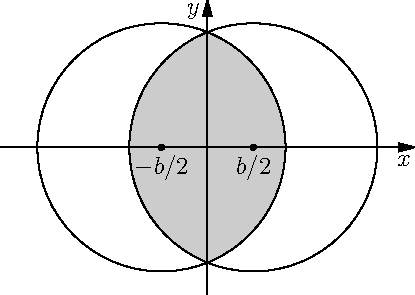
\includegraphics{fig1.eps}}
\caption{The dependencies of magnetic field $eB$ (at central point $(x, y) = (0, 0)$ )on proper time $\tau$ at $\sqrt{s_{NN}}$ = 2760 GeV(a) for Pb-Pb collisions
and 200 GeV for Au-Au collisions with b = 8 fm, respectively. The solid line and dashed line are for the consideration of response of QGP medium and in the vacuum with no
response of QGP medium, respectively.}
\label{fig1} %Fig.1
\end{figure}

Fig. 2(a) shows the comparison between our calculated magnetic field $eB$ and Skokov's calculation results. The real line is our calculation results, the dotted line is from
Skokov's calculation results with realistic Lattice QCD electrical conductivity~\cite{lab19} and the dash-dotted line is from Skokov's calculation results in the vacuum. We also find
that magnetic field with the consideration of response of QGP medium decreases more slowly than that of in the vacuum. Fig. 2(b) shows the comparisons
between our calculated magnetic field $eB$ and Tuchin's calculation results. The real line is our calculation results, the dotted line is from
Tuchin's calculation results with electrical conductivity $\sigma=5.8$ MeV~\cite{lab17}, the dash-dotted line is from Tuchin's  extensive study the magnetic field~\cite{lab21}
and dashed line is from Tuchin's calculation results in the vacuum. In our analysis, we take the ideally conducting limit with Bjorken space time evolution mechanism.

\hskip0.2cm

\begin{figure}[h!]
\centering \resizebox{0.4\textwidth}{!}{
\includegraphics{fig2.eps}}
\caption{The comparisons among our calculated magnetic field $eB$ with Skokov's(a) and Tuchin's(b) calculation results of magnetic field $eB$.}
\label{fig2} %Fig.2
\end{figure}


\section{The calculations of chiral charge separation }
For each event, one defines~\cite{lab29}
\begin{eqnarray}
g(\phi_{s},\phi_{t})=\frac{1}{N_{s}N_{t}}\sum_{i=0}^{N_{s}}\sum_{i=0}^{N_{t}}\textrm{cos}(\phi_{si}+\phi_{ti}),
\label{eq:eq24} %Eq.24
\end{eqnarray}

\noindent where $s,t=\pm$ denotes the charge sign, $\phi_{si}$
denotes the azimuthal angle of an individual charged particle with respect to the reaction plane, and $N_{\pm}$ is the total number of positively or negatively charged particle.

Then one can average the correlators over $N_{e}$ similar events to remove the multiplicity fluctuations. One can define the averaged
correlators $a_{++}$, $a_{--}$, $a_{+-}$ and $a_{-+}$~\cite{lab7,lab29} as
\begin{eqnarray}
a_{st}=-\frac{1}{N_{e}}\sum_{n=1}^{N_{e}}g(\phi_{s},\phi_{t}).
\label{eq:eq25} %Eq.25
\end{eqnarray}

The correlators can also be given as
\begin{eqnarray}
g(\phi_{s},\phi_{t})=\frac{1}{N_{s}N_{t}}(X_{s}X_{t}-Y_{s}Y_{t}),
\label{eq:eq26} %Eq.26
\end{eqnarray}

\noindent where
\begin{eqnarray}
X_{\pm}\equiv\sum_{i=1}^{N_{\pm}}\textrm{cos}(\phi_{i}^{\pm}),~~~~~~~Y_{\pm}\equiv\sum_{i=1}^{N_{\pm}}\textrm{sin}(\phi_{i}^{\pm})
\label{eq:eq26} %Eq.26
\end{eqnarray}

If all charged particles would be really emitted perpendicular to the reaction plane in which case $\phi=\pi/2$ or ��$\phi=3\pi/2$,
we will have
\begin{eqnarray}
Y_{\pm}=\Delta_{\pm}.
\label{eq:eq27} %Eq.27
\end{eqnarray}

One should note that for vanishing net charge density per unit rapidity at $\eta$ = 0, the invariance under charge transformation predicts that
$a_{++}=a_{--}$, and $a_{+-}=a_{-+}$. RHIC and LHC experiments carried out a series of studies of chiral
charge separation effect~\cite{lab8,lab9,lab10,lab11}, we also look for clues related to the effects.
In order to look for whether the signal seen in Ref.~\cite{lab8,lab9,lab10,lab11} is really due to the chiral magnetic effect one has to perform a detailed
analysis and see whether calculations based on the chiral magnetic effect are consistent with the data.

As a result, we would have
\begin{eqnarray}
a_{++}=a_{--}=\frac{1}{N_{+}^{2}}<\Delta_{\pm}^{2}>,
\label{eq:eq28} %Eq.28
\end{eqnarray}

\noindent and
\begin{eqnarray}
a_{+-}=a_{-+}=\frac{1}{N_{+}N_{-}}<\Delta_{+}\Delta_{-}>,
\label{eq:eq29} %Eq.29
\end{eqnarray}

\noindent where $N_{\pm}$ denotes the total number of charged particles in the related $\eta$
interval.

\begin{figure}[h!]
\centering \resizebox{0.45\textwidth}{!}{
\includegraphics{fig3.eps}}
\caption{The dependencies of $a_{++}$($a_{--}$) on centralities for Au - Au collisions at $\sqrt{s_{NN}}$ = 200 GeV(a)
of RHIC energy region, and for Pb - Pb collisions at $\sqrt{s_{NN}}$ = 2760 GeV(b) of LHC energy region for different values of the screening length $\lambda$.}
\label{fig3} %Fig.3
\end{figure}

Refs.~\cite{lab30,lab31} published some  geometrical properties of the collision, such as the number of
participating nucleons and the number of binary nucleon-nucleon collisions, which are deduced from a Glauber model with a sharp impact parameter selection and shown to be consistent
with those extracted from the data of RHIC and LHC energy regions. Fig. 3(a, b) show the dependencies $a_{++}$($a_{--}$) of the chiral magnetic effect as a function of centrality,
for Au - Au collisions at $\sqrt{s_{NN}}$ = 200 GeV(a) of RHIC energy region, and for Pb - Pb collisions at $\sqrt{s_{NN}}$ = 2760 GeV(b) of LHC energy region with different values of the screening length $\lambda$ = 0.1R, 0.2R and 0.3R, respectively. One find that $a_{++}$ increases with the increase of centralities. One also find that $a_{++}$ increases with the increase of nuclear screening length.
Our result for $a_{++}$ and $a_{+-}$ is displayed in Fig.3. Qualitatively the result agrees with the data presented in Ref.~\cite{lab8,lab9,lab10,lab11}.

\begin{figure}[h!]
\centering \resizebox{0.45\textwidth}{!}{
\includegraphics{fig4.eps}}
\caption{The result of the correlator $|a_{+-}|/a_{++}$ as a function of $b/R$ for Au - Au collisions at $\sqrt{s_{NN}}$ = 200 GeV (a)
of RHIC energy region, and for Pb - Pb collisions at $\sqrt{s_{NN}}$ = 2760 GeV (b) of LHC energy region for different values of the screening length $\lambda$.}
\label{fig4} %Fig.4
\end{figure}

We showed $|a_{+-}|/a_{++}$ as a function of $b/R$ in Fig.4 for different values of $\lambda$. To calculate  $a_{+-}$ and $a_{++}$
we used the screening suppression factor $f_{\pm}(x_{\perp})$ given in
Eq.(4). It is found that the suppression of $a_{+-}$ compared to $a_{++}$ decreases with the increase of impact parameter. This is because the system size is smaller
in larger impact parameter.

\begin{figure}[h!]
\centering \resizebox{0.45\textwidth}{!}{
\includegraphics{fig5.eps}}
\caption{Comparison of $a_{++}$($a_{--}$)(a) of the chiral magnetic effect as a function of centralities with different screening length between Au - Au collisions
 and that of Cu - Cu collisions at $\sqrt{s_{NN}}$ = 200 GeV. Comparison of $|a_{+-}|/a_{++}$ (b) of the chiral magnetic effect as a function of centralities
with different screening length between Au - Au collisions  and that of Cu - Cu collisions at $\sqrt{s_{NN}}$ = 200 GeV.}
\label{fig5} %Fig.5
\end{figure}

Fig.5(a) compares of $a_{++}$($a_{--}$) of the chiral magnetic effect as a function of centralities with different
screening length in Au - Au collisions at $\sqrt{s_{NN}}$ = 200 GeV with that of Cu - Cu collisions. One finds that the
smaller the collision system, the larger the $a_{++}$($a_{--}$) is.  On the contrary, a comparison of $|a_{+-}|/a_{++}$  in Fig. 5 (b) as a function of centralities
with different screening length between Au - Au collisions at $\sqrt{s_{NN}}$ = 200 GeV and that of Cu - Cu collisions indicates that $|a_{+-}|/a_{++}$ is larger for larger collision system.


% \begin{figure}[h!]
% \centering \resizebox{0.45\textwidth}{!}{
% \includegraphics{fig6.eps}}
% \caption{$a_{++}$($a_{--}$)(a) and $a_{+-}$($a_{-+}$)(b) of the chiral magnetic effect as a function of centralities for different collision energies
% at $\sqrt{s_{NN}}$ = 62.4 GeV, 130GeV, 200GeV and 2760 GeV of RHIC and LHC energy regions for the screening length $\lambda/R$ = 0.3.}
% \label{fig6} %Fig.6
% \end{figure}

Fig.6 shows the dependencies of $a_{++}$($a_{--}$)(a) and $a_{+-}$($a_{-+}$)(b) on the centralities with different collision energies
of $\sqrt{s_{NN}}$ = 62.4 GeV, 130 GeV, 200 GeV and 2760 GeV in the RHIC and LHC energy regions for the screening length $\lambda/R$ = 0.3. It is found that
the chiral separation effect increases with the impact parameter increases. The chiral separation effect approaches zero at central collisions and
the maximum value of the chiral separation effect can reach $1.8\times10^{-3}$ when centrality $70\%-80\%$ and the screening length $\lambda/R$ = 0.3.

% \begin{figure}[h!]
% \centering \resizebox{0.45\textwidth}{!}{
% \includegraphics{fig7.eps}}
% \caption{$<\Delta_{\pm}^{2}>$(a) and $<\Delta_{+}\Delta_{-}>/<\Delta_{\pm}^{2}>$ (b) of the chiral magnetic effect as a function of centralities for different collision energies
% at $\sqrt{s_{NN}}$ = 62.4 GeV, 200GeV and 2760 GeV of RHIC and LHC energy regions for the screening length $\lambda/R$ = 0.2.}
% \label{fig7} %Fig.7
% \end{figure}

Fig.7(a) shows the dependencies of $<\Delta_{\pm}^{2}>$ of the chiral magnetic effect as a function of centralities for different collision energies
at $\sqrt{s_{NN}}$ = 62.4 GeV, 200GeV and 2760 GeV of RHIC and LHC energy regions. It is found that $<\Delta_{\pm}^{2}>$ is larger at LHC energy
region $\sqrt{s_{NN}}$ = 2760 GeV than that RHIC energy region $\sqrt{s_{NN}}$ = 62.4 GeV and 200GeV , and the $<\Delta_{\pm}^{2}>$ is almost the same in the RHIC energy region.

Fig.7(b) shows the dependencies of $<\Delta_{+}\Delta_{-}>/<\Delta_{\pm}^{2}>$ of the chiral magnetic effect as a function of centralities for different collision energies
at $\sqrt{s_{NN}}$ = 62.4 GeV, 200GeV and 2760 GeV of RHIC and LHC energy regions. It is found that $<\Delta_{\pm}^{2}>$ is slightly smaller at that $\sqrt{s_{NN}}$ = 2760 GeV of LHC
energy region than that of  $\sqrt{s_{NN}}$ = 62.4 GeV and 200GeV of RHIC energy region, and the $<\Delta_{+}\Delta_{-}>/<\Delta_{\pm}^{2}>$ at $\sqrt{s_{NN}}$ = 62.4 GeV and 200GeV in
the RHIC energy region is almost the same.


\section{Summary and Conclusion}
In this paper, we study systematically the dependencies of chiral charge separation on centralities, collision energies and collision nuclei in the RHIC and LHC energy regions.
The response of QGP medium to magnetic field is introduced to study the features of chiral magnetic field  in relativistic heavy-ion collisions.
In our analysis, we take the ideally conducting limit with Bjorken space time evolution mechanism and neglect the diffusion terms. We take a different
method from these popular Tuchin's and Skokov's methods on the issue of dealing with the problem of QGP media response in this paper.

The dependencies $a_{++}$ of the chiral magnetic effect as a function of centrality in the RHIC and LHC energy regions for different values of the screening length $\lambda$ are given in this paper. It is
found that $a_{++}$ increases with the increase of impact parameter and nuclear screening length.  Qualitatively our results agree with the data presented in Ref.~\cite{lab8,lab9,lab10,lab11}.
It is found that nuclear screening effect has an important influence on the chiral charge separation characteristics.

We make a comparison between $a_{++}$ of the chiral magnetic effect as a function of centralities with different
screening length of Au - Au collisions at $\sqrt{s_{NN}}$ = 200 GeV and that of Cu - Cu collisions. It is shown that the
smaller the collision system, the larger the $a_{++}$($a_{--}$) is.  We also make a comparison between $|a_{+-}|/a_{++}$  of the chiral magnetic effect as a function of centralities with different screening length of Au - Au collisions at $\sqrt{s_{NN}}$ = 200 GeV and that of Cu - Cu collisions. It is found that $|a_{+-}|/a_{++}$ of the  larger Au - Au collision system is larger than that of smaller Cu - Cu collision system.

We also find that the chiral separation effect increases with the impact parameter increases. The chiral separation effect approaches zero at central collisions and
the maximum value of the chiral separation effect can reach $1.8\times10^{-3}$ when centrality $70\%-80\%$ and the screening length $\lambda/R$ = 0.3 in the RHIC and LHC energy regions.


\section{Acknowledgments}
This work was supported by National Natural Science Foundation of China (Grant Nos: 11475068, 11247021, 11447023), the CCNU-QLPL Innovation Fund (Grant No: QLPL2014P01),
the Excellent Youth Foundation of Hubei Scientific Committee (Grant No: 2006ABB036).


\begin{thebibliography}{}
\bibitem{lab1} T. D. Lee, Phys. Rev. D 8, 1226 (1973); T.D. Lee and G. C. Wick, Phys. Rev. D 9, 2291 (1974).
\bibitem{lab2} P. D. Morley and I. A. Schmidt, Z. Phys. C 26, 627 (1985).
\bibitem{lab3} D. Kharzeev, R. D. Pisarski, and M. H. G. Tytgat, Phys.Rev. Lett. 81, 512 (1998); D. Kharzeev and R. D. Pisarski,
Phys. Rev. D 61, 111901 (2000).
\bibitem{lab4} T. Scha$\ddot{a}$fer and E.V. Shuryak, Rev. Mod. Phys. 70, 323 (1998).
\bibitem{lab5} S. S. Chern and J. Simons, Ann. Math. 99, 48 (1974).
\bibitem{lab6} D. Kharzeev, Phys. Lett. B 633, 260 (2006); K. Fukushima, D. E. Kharzeev, and H. J. Warringa, Phys.
Rev. D 78, 074033 (2008).
\bibitem{lab7} D. Kharzeev, L. D. McLerran, and H. J. Warringa, Nucl. Phys. A803, 227 (2008).


\bibitem{lab8} STAR Collaboration, Abelev B I et al., Phys. Rev. Lett. 103, 251601 (2009).
\bibitem{lab9} STAR Collaboration, B. I. Abelev et al., Phys. Rev. C 81, 054908 (2010).
\bibitem{lab10} STAR Collaboration, Selyuzhenkov I V, Romanian Reports in Physics. 58, 49 (2006).
\bibitem{lab11} ALICE Collaboration, B. I. Abelev et al., Phys. Rev. Lett. 110, 012301(2013).
\bibitem{lab12} Y. J. Mo, S. Q. Feng, and Y. F. Shi,  Phys. Rev. C 88,  024901(2013).
\bibitem{lab13} Y. Zhong, C.-B. Yang, X. Cai, and S.-Q. Feng, Adv. High Energy Phys. 2014, 193039(2014); Y. Zhong, C.-B. Yang, X. Cai, and S.-Q. Feng, Chinese Physics C 39, 104105 (2015).
\bibitem{lab14} V. Voronyuk, V. D. Toneev, W. Cassing, E. L. Bratkovskaya, V. P. Konchakovski, and S. A. Voloshin, Phys. Rev. C 83, 054911 (2011).
\bibitem{lab15} V. Skokov, A. Y. Illarionov, and V. Toneev, Int. J. Mod. Phys. A24, 5925 (2009).
\bibitem{lab16} W. T. Deng, and X. G. Huang, Phys. Rev. C 85, 044907 (2012).
\bibitem{lab17} K. Tuchin,  Adv. High Energy Phys. 2013, 490495(2013).
\bibitem{lab18} K. Tuchin, Phys. Rev. C 88, 024911(2013).
\bibitem{lab19} L. McLerran, V. Skokov, Nucl. Phys. A929, 184 (2014).
\bibitem{lab20} K. Tuchin, Phys. Rev. C 91, 064902 (2015)
\bibitem{lab21} K. Tuchin, Phys. Rev. C 93, 014905 (2016).
\bibitem{lab22} H. Li, X.-L Sheng, and Q. Wang Phys. Rev. C 94, 044903 (2016).
\bibitem{lab23} L.D. McLerran, E. Mottola, M.E. Shaposhnikov, Phys. Rev. D 43, 2027 (1991).
\bibitem{lab24} G.D. Moore, C.R. Hu, B. Muller, Phys. Rev. D 58,  045001 (1998).
\bibitem{lab25} D. B$\ddot{o}$deker, G.D. Moore, K. Rummukainen, Phys. Rev. D 61, 056003 (2000).
\bibitem{lab26} H. T. Ding, A. Francis, O. Kaczmarek, F. Karsch, E. Laermann,and W. Soeldner, Phys. Rev. D 83, 034504 (2011).
\bibitem{lab27} J. D. Bjorken, Phys. Rev. D 27, 140 (1983).
\bibitem{lab28} J. Y. Ollitrault, Eur. J. Phys. 29, 275 (2008).
\bibitem{lab29} S.A. Voloshin, Phys. Rev. C 70, 057901 (2004).
\bibitem{lab30} ALICE Collaboration, B. I. Abelev et al., Phys. Rev. C 88, 044909(2013).
\bibitem{lab31} STAR Collaboration, B. I. Abelev et al., Phys. Rev. C 79, 034909 (2009).
\end{thebibliography}{}

\end{document}
